\chapter{NAPT}

プロキシとNAT、それぞれにメリットとデメリットがありました。外のネットワークと直接通信したい。
そんな要求がなくなることはありません。

そこで考案されたのが、第三の方法であるNAPTです。IPv4のネットワークにでは大抵使われているNAPTは、どのような技術なのでしょうか。

\section{ホストよるグローバルのIPアドレスが少ない}
静的NATを使えば、任意のプロトコルで外部のホストと対等に通信することができる。
だが、通信を行うホストと同じ数のグローバルなIPアドレスが必要となる。だが、それだけのグローバルIPアドレスが準備できないことが多い。

動的NATを使用したとしても、アドレスのマッピングが一定しないこと、TCPのKeepalieとの相性が良くないこと、などのいくつかの問題がある。

一方のアプリケーション層のプロキシは、クライアント・サーバ型通信に限られるが、ひとつのプロキシで複数のクライアントのリクエストを中継することができる。

では、NATとプロキシのいいとこ取りをすることはできないか、それを考えてみよう。


\section{NAPT}

\begin{figure}[htbp]
	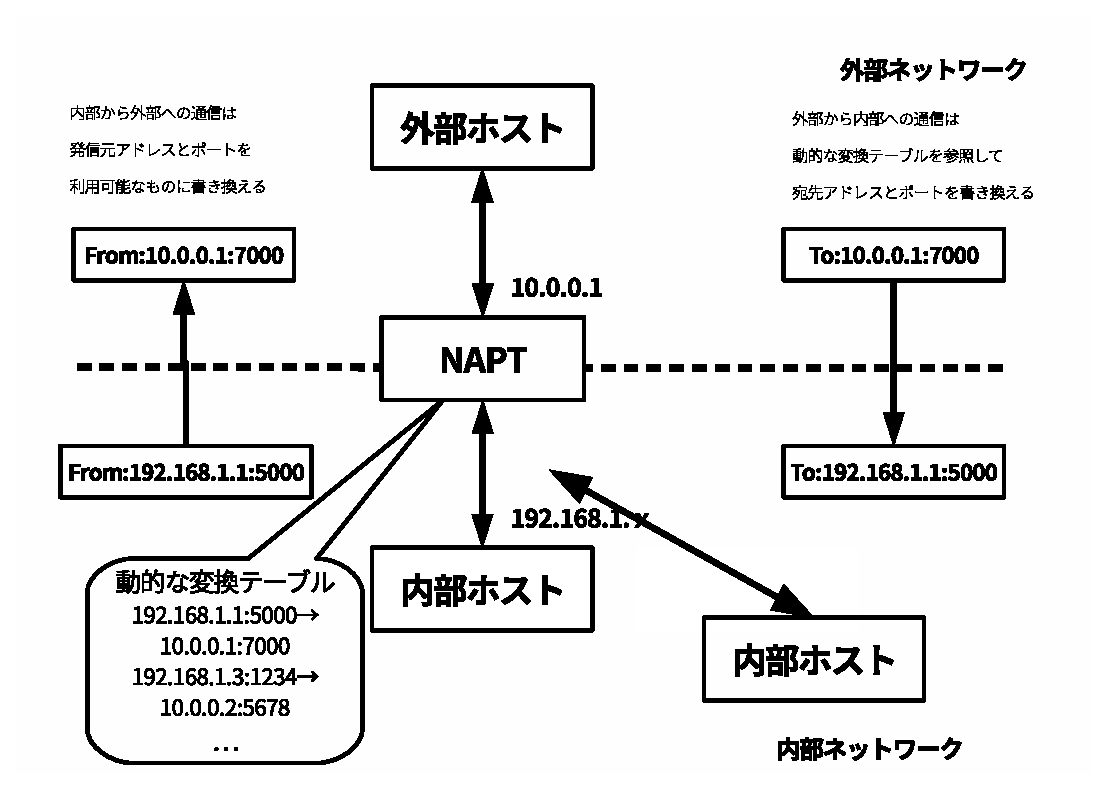
\includegraphics[width=12cm,clip]{draw/fig9.eps}
	\caption{NAPT}
	\label{fig:NAPT}
\end{figure}

まず、グローバルなIPアドレスが一つしか無い状況で、任意のアプリケーションと通信をしたい、という要求にどう答えればいいか、それを考えてみる。

プロキシは、グローバルなIPアドレスがひとつでも使用できる。だが、任意の通信を行いたいので、プロキシは利用できない。
逆に、静的NATは、任意の通信ができるが、グローバルなアドレスがホストの数だけ必要となる。
では、なぜ静的NATは、グローバルなアドレスがホストの数だけ必要となるのだろうか。理由か簡単で、ポート番号の変換を行っていないため、IPアドレスを多重に使うことができないからだ。

トランスポート層のポート番号は、元々ひとつのIPアドレスを多重に使うために導入された技術であった。これは、ひとつのホストが、多重にほかのプロセスと通信するための手段であったわけだ。

では、この、多重化の考えをNATにも導入してみよう。通信のイニシエイターであるホストのIPアドレスとポート番号をセットにして、ルータで記録する。そして、ルータでは、発信元のIPアドレスをグローバルのIPアドレスに書き換えるl。そして、変換後のIPアドレスで、未使用のポートを発信ポートとするようにトランスポート層のヘッダも書き換える。

サーバからのレスポンスは、ルータで変換したIPアドレスとポートを宛先として送信される。ルータは、インターネットプロトコル層のヘッダと、トランスポート層のヘッダを記録と引きあわせる。

そして、記録にある、該当するリクエストの発信元IPアドレスを、インターネットプロトコル層のヘッダの宛先IPアドレスとして書き換える。同様に、記録にある発信元ポート番号を、トランスポート層のヘッダの宛先ポートとして書き換える。

こうすることで、内部から外部に、任意の通信を行うことができる。ルータで変換した後のポート番号は空いているところを使う。
このように、内部ホストのアドレス、ポートと送出するときのポートのマッピングを動的に行うことから、NATとの対比で、NAPT(Network Address and Port Translate)と呼ぶ。

\subsection{NATPのメリットとデメリット}
NAPTの内部処理は複雑で、比較的重い。では、この処理を入れることによる、メリットとデメリットは何であろうか。メリットは、動的NATと比較して、より多くの内部ホストが、同時に外部と通信できることである。

一方、デメリットは、使用可能なポートの数、つあり、理論でいけば約65000のセッションまでしか通信できないという点である。
この数字は、一見すると多い。だが、Ajaxなど、同時に多数のセッションを必要とするホストが内部に多数あれば、この数字を束果たす可能性がある。

また、NAPTは、変換のために、ルータのCPUやメモリといったリソース消費する。トランスポートスのヘッダ、インターネットプロトコル層のヘッダを書き換え、トランスポート層のチェックサムを再計算し、トランスポート層のヘッダを再構成する。そのため、内部ホストの台数に応じた性能のルータを必要とする。


\subsection{NAPTの名前}
NAPTにも、実装毎にいくつかの呼び方がある。LinuxなどではIP Masquaradeであり、PAT(Port Address Translate)という呼び方をする実装もある。また、単にNATと呼んだとき、暗黙のうちにNAPTを指すこともある。

ただし、NAPTと、前の章で説明した動的NATが混同されている場合がある。動的NATという言葉が使われているときは、ポート変換の有無を見て判断する必要がある。

\section{NAPTの通信の方向}

NAPTを使えば、中から外への任意の通信が行えることはわかった。だが、外から中への通信はどうだろうか。それを考えてみよう。

\subsection{外から中への通信}
結論を述べれば、外のホストがイニシエイターになる、中への通信ができない。正確には、外のホストがイニシエイターとなる通信で、中のホストを特定する方法がない。

内部のホストがイニシエイターとなって、外部に行った通信のレスポンスはルータに到達しすると、その発信元のIPアドレスと、宛先のポート番号を、ルータの変換テーブルと比較される。そうすることで、最終的にNAPTは送り先の内部ホストが決定する。

だが、外部ホストがイニシエイターである通信の場合、この変換テーブルの記録が存在しない。そのため、宛先を特定できず、通信が成立しないことにある。そのため、NAPTは、クライアント・サーバ型の通信で、内部がクライアントとなる形態でにのみ使用できる。

\subsection{ポートフォワーディング}

\begin{figure}[htbp]
	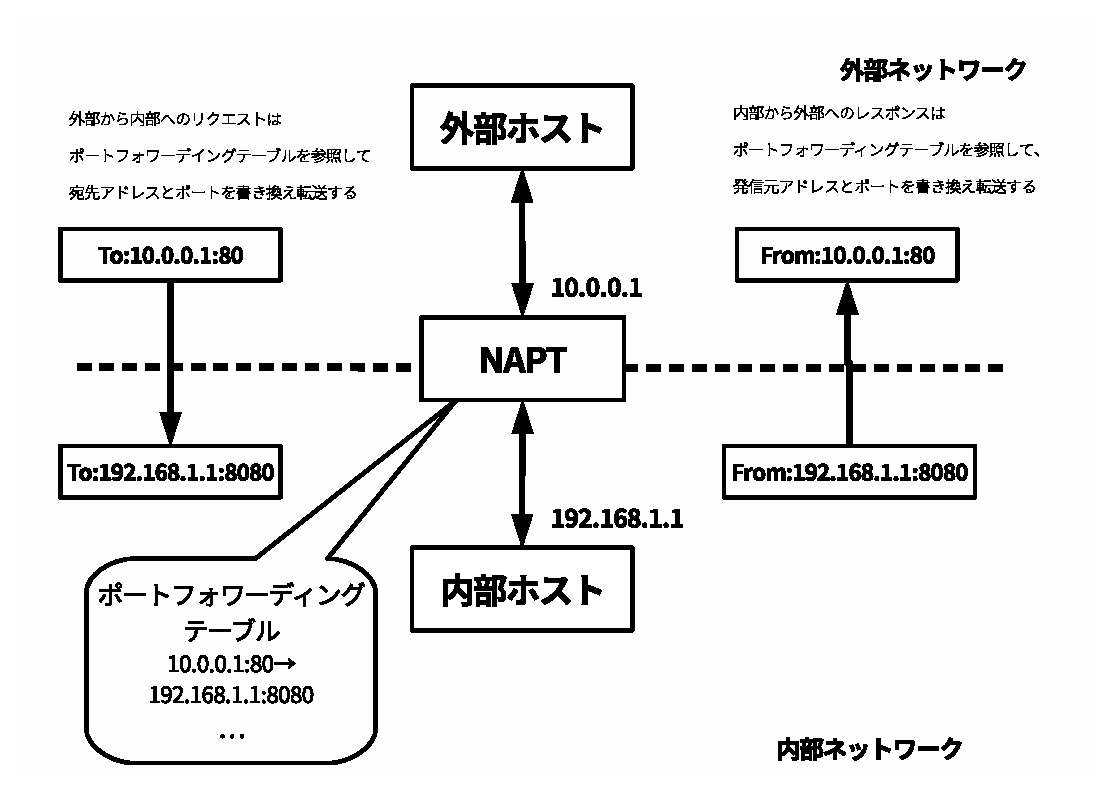
\includegraphics[width=12cm,clip]{draw/fig10.eps}
	\caption{ポートフォワーディング}
	\label{fig:port-forward}
\end{figure}

NAPTは、外部ホストがイニシエイターとなる通信はできない。これは、到達した通信が、内部のどのホスト喉のポート宛であるかを特定する、変換テーブルの情報がないためである。
逆に言えば、この変換情報を予め用意できれば、内部の特定のホストの、特定のポートに対しての通信をすることはできる。

外側になるグローバルIPアドレスとポートを予約する。このアドレスとポートを宛先とする通信があれば、予め設定されていた通り、内部ホストの特定のポートを宛先とするようにヘッダ情報を書き換えて送信する。

このように、外部からのアクセスは、特定のホストの特定のポートに対して通信を転送する。そのため、ポートフォワーディングと呼んでいる。

\subsection{NAPTはセキュリティか}
このように、外部から内部にアクセスしづらい性質から、NAPTはセキュリティのためのものとして説明されることがある。\footnote{それ故にIPv6をNATを使わないことでセキュリティを低下させると論ずる説明まである。困ったものだ。}
だが、NAPTは、本質的に、セキュリティのための仕組みではない。

NAPTをセキュリティを目的として使用するとすれば、それは大きな間違いである。ポートフォワーディング設定がされていれば内部のホストにアクセスすることは可能である。また、NAPTから外の通信ををキャプチャして解析すれば、変換テーブルに従って内部に届けられるデータグラムを生成し、攻撃のために送り込むすることが可能である。

このように、NAPTを使ってもセキュリティという観点からは何の役にも立たない。

\section{デュアルスタックとNAPT}
NAPTは、多くの場合、インターネットプロトコル層がIPv4であるときに使用される。これは、割当数の少ないグローバルのIPv4アドレスを多重化して、多くのクライアントで強要しようという仕組み仇からだ。

IPv6のULAとGUAの間の変換に使用数r湖とも、技術的には可能である。だが、IPv6のGUA配布がネットワークアドレス単位で行われる現状は、実用的な意味が無い。

\subsection{NAT64}

IPv6が使うNAPTの例外が、NAT64という、IPv6のみのホストが、IPv4のアドレスを持つホストにアクセスするための変換である。NAT64は、内側ネットワークがIPv6、外側がIPv4のNAPTである。

NAT64は、DNS64というDNSリゾルバを使用する。DNS64は、名前解決のリクエストを受けると、IPv6のアドレスで解決可能なら、そのままIPv6のアドレスをクライアントに返す。この場合、クライアントは、IPv6のアドレスを使って目的のホストにアクセスする。このとき、NAPTもしくはNATで行うようなアドレス変換は行われない。ネイティブのIPv6アクセスが行われる。

DNS64は、IPv4でしかアクセスができないホストの名前解決をしたときは、そのIPv4アドレスをベースに、プレフィクスを付加して識別刷ることが可能なIPv6アドレスを生成し、クライアントに返す。
IPv6のホストは、そのアドレスを宛先として、ゲートウェイとなるルータ経由でインターネットにアクセスしようとする。この時のゲートウェイがNAT64となる。

このプレフィクスがついた、IPv6の宛先アドレスを持つIPデータグラムを受け取ったNAT64は、宛先アドレスからIPv4アドレスを取り出し、必要ならトランスポート層のチェックサム計算を行って、IPv4のデータグラムに変換する。
そして、自分が始点となって、IPv4のアクセスを行う。この動作は、NAPT的な動作である。

そして、その応答は、NAT64がヘッダをIPv6にして、トランスポート層のチェックサムがあれば計算し直し、IPv6のデータグラムに再構築してアクセス元のホストに送る。
IPv6は必ずPMTUをおこなう。そのため、途中の経路でフラグメントが発生するようなMSSにはならない。これは、IPv6のヘッダがIPv4のヘッダよりもサイズが大きいことから自明である。